\documentclass[12pt]{article}
\usepackage[utf8]{inputenc}
\usepackage[a4paper, margin=2cm]{geometry}
\usepackage{multicol, caption}
\usepackage{authblk}
\usepackage[varg]{txfonts}
\usepackage{titlesec}
%\usepackage[T1]{fontenc}
%\usepackage{lmodern}
% \usepackage[english]{babel}


\usepackage{amsmath}
\usepackage{amssymb}
\usepackage{amsfonts}
\usepackage{graphicx}% Include figure files
\usepackage{dcolumn}% Align table columns on decimal point
\usepackage{bm}% bold math
\usepackage{hyperref}% add hypertext capabilities
\usepackage{minted}
\usepackage[autostyle]{csquotes}

\usepackage[backend=biber,style=numeric]{biblatex}
\addbibresource{bib.bib}

\hyphenpenalty=10000
\exhyphenpenalty=10000

% CUSTOM FORMAT FOR SECTION
\titleformat{\section}[wrap]{\normalfont\bfseries}{\thesection.}{0.5em}{}
\titlespacing{\section}{12pc}{1.5ex plus .1ex minus .2ex}{1pc}
% CUSTOM SUBSECTION
\titleformat{\subsection}[wrap]{\normalfont\bfseries}{\thesubsection.}{0.5em}{}
\titlespacing{\subsection}{12pc}{1.5ex plus .1ex minus .2ex}{1pc}
% CUSTOM SUBSUBSECTION 
\titleformat{\subsubsection}[wrap]{\normalfont\bfseries}{\thesubsubsection.}{0.5em}{}
\titlespacing{\subsubsection}{12pc}{1.5ex plus .1ex minus .2ex}{1pc}

% CUSTOM LINE SPACING (Default 1.2 -> 1.2*1.25=1.5)
\linespread{1.25}

% CUSTOM NAMING
\renewcommand*\contentsname{Summary}

\newenvironment{Figure}
  {\par\medskip\noindent\minipage{\linewidth}}
  {\endminipage\par\medskip}

\title{PHYS6006 Final Report \\
       Magnetospheric structure associated with high-latitude auroras}
\author[1]{J. Plank}
\author[2]{R. C. Fear}
\affil[1, 2]{Department of Physics and Astronomy, University of Southampton}
\date{April 2020}

\begin{document}\sloppy
% TITLE BLOCK
\maketitle

% ABSTRACT
\begin{abstract}
    \noindent\textit{Context:} Only case studies have been done on the magnetospheric structure associated with the formation of high latitude aurora, and the connection of interplanetary magnetic field direction is suspected but has never been quantified.\\
    \textit{Aims:} To produce a statistical survey on the relationship between a northward pointing interplanetary magnetic field and a phenomenon known as transpolar arcs.\\
    \textit{Methods:} Using data from the ESA satellite Cluster, we analysed the ion temperature for many different values of $Z_{GSM}$, covering the plasma sheet as well as the magnetotail lobes.\\
    \textit{Results:} We found a direct link to IMF direction based on high temperature events observed in the lobe, suggesting high-latitude aurora form during periods of northward pointing IMF.
\end{abstract}

\pagebreak

\tableofcontents
\addtocontents{toc}{~\hfill\textbf{Page}\par}
\addtocontents{lof}{~\hfill\textbf{Page}\par}
\bigskip
\listoffigures

\pagebreak

% % SWITCH TO 2 COLUMNS
% \begin{multicols}{2}

\section{INTRODUCTION}
Earth and the Sun are connected by more than just gravity, magnetic interactions between the two bodies are the cause of some of the most dramatic and complex phenomena on Earth. The most well known of these is the aurora (Borealis in the northern hemisphere and Australis in the southern). More commonly known as the northern and southern lights, these light shows come as a result of charged particles flowing along the Sun's magnetic field lines (known as solar wind) and making their way down to Earth in a zone known as the auroral oval \cite{AAAspaceweather}. The Sun's violent nature is also transmitted to Earth along its magnetic field, known as the `Interplanetary magnetic field` (IMF). This can result in satellite damage, radiation hazards to astronauts and airline passengers, telecommunications problems, and outages of power and electronics systems \cite{AAAspaceweather}.

The modern theory of the formation of the aurora was first proposed by Kristian Birkeland in 1903 \cite{birkeland2018norwegian}. He said that auroras are produced when solar wind encounters the geomagnetic field. The result of this is the formation of the plasmasphere in the equatorial plane of Earth's magnetic field \cite{cosmicelectrodyn}.

\subsection{Structure of Earth's magnetic field}
Figure \ref{fig:plasmasphere} is a representation of the solar-terrestrial environment. The solar wind, travelling with the interplanetary magnetic field from the sun \cite{Svalgaard_2010}, is coming from the left. It collides with the terrestrial magnetic field at supersonic speeds, creating a bow shock wave in front of the magnetosphere - the region where magnetic field lines connect to Earth at both ends - the boundary of the magnetosphere is the magnetopause. Supersonic solar winds compress at this boundary creating a magnetosheath between the magnetopause and the bow shock \cite{BSPP}.

\begin{Figure}
    \begin{minipage}[c]{0.57\textwidth}
        \centering
        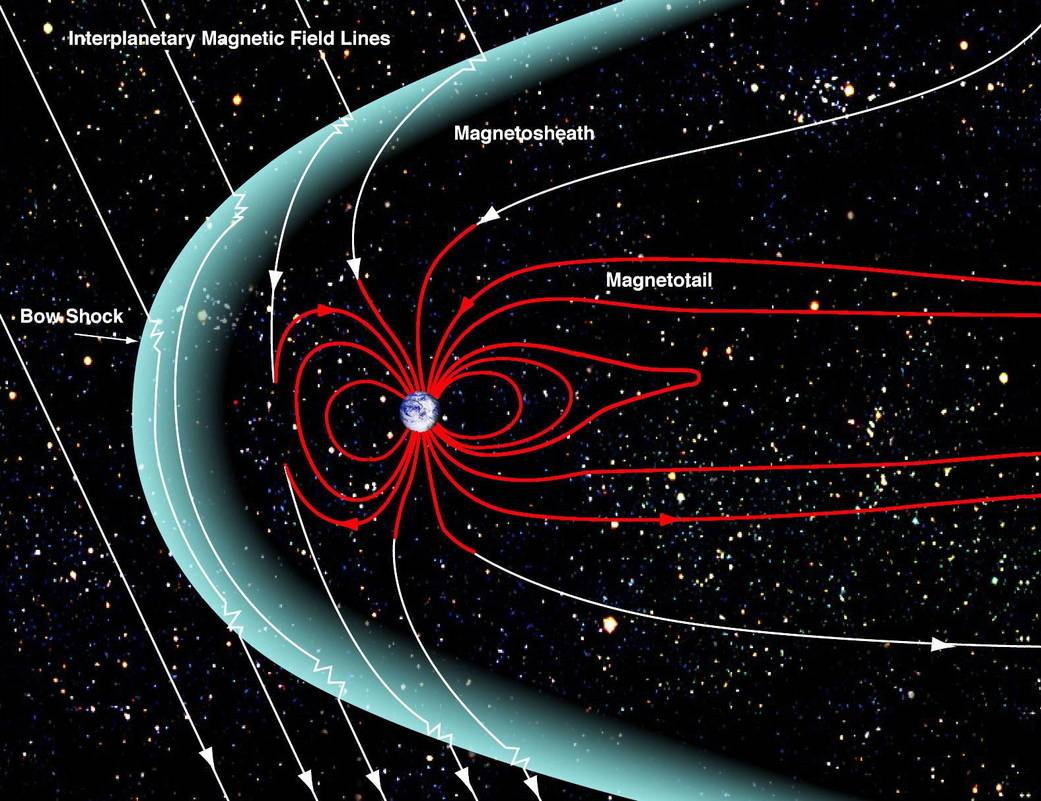
\includegraphics[width=0.7\textwidth]{NASA-Magnetosphere.jpeg}
    \end{minipage}\hfill
    \begin{minipage}[c]{0.4\textwidth}
        \captionof{figure}{Representation of the solar-terrestrial magnetic interaction. The sun is located to the left, producing solar winds and the IMF. Solar winds collide with the terrestrial magnetic field at supersonic speeds, creating a bow shock wave which encases the magnetosphere in a magnetosheath of compressed solar wind \cite{BSPP}. (Image courtesy of NASA)}
        \label{fig:plasmasphere}
    \end{minipage}
\end{Figure}

\subsection{Coordinate Systems}
Geocentric Solar Ecliptic (GSE) and Geocentric Solar Magnetic (GSM) are two similar coordinate systems used when studying the magnetosphere. Both have the Earth as the origin, and $+X$ pointing towards the sun. In GSE, $+Z$ is pointed perpendicularly upwards from the plane of Earth's orbit around the Sun. In GSM, $Z$ is the projection of Earth's magnetic dipole axis onto the plane perpendicular to $X$, with positive pointing north.

\begin{Figure}
    \begin{minipage}[c]{0.48\textwidth}
        \centering
        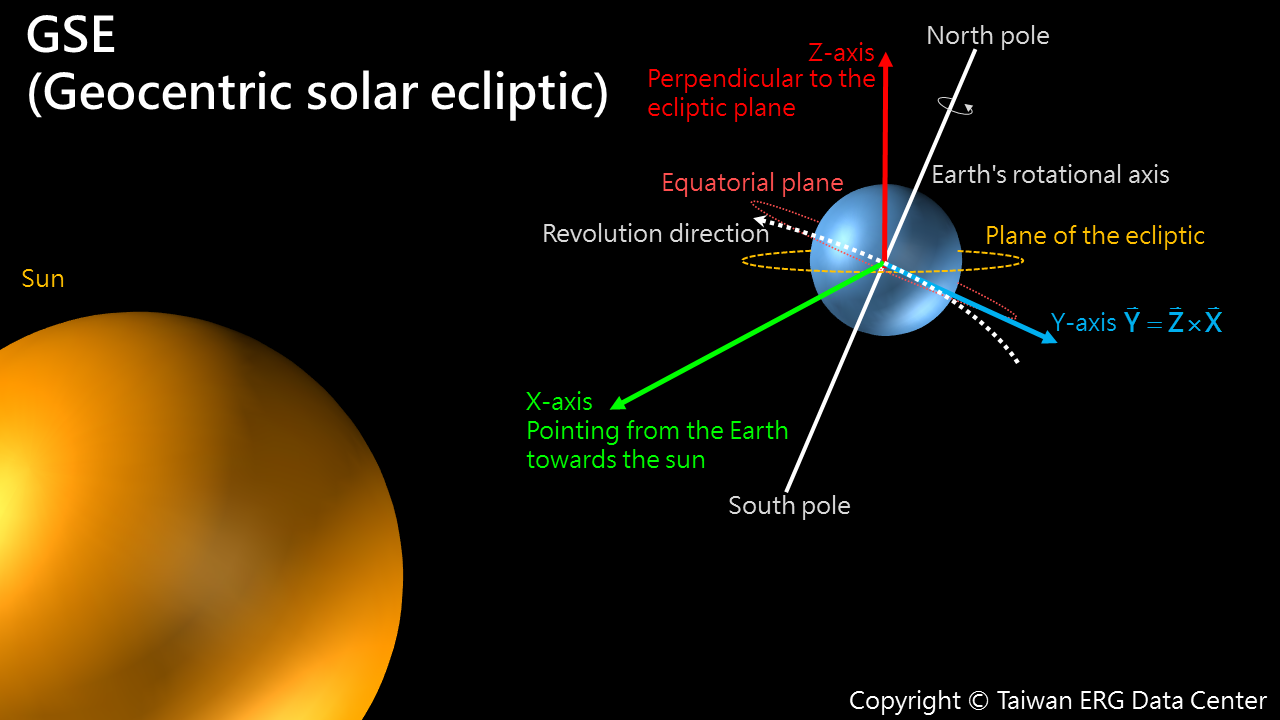
\includegraphics[width=\textwidth]{GSE.png}
    \end{minipage}
    \begin{minipage}[c]{0.48\textwidth}
        \centering
        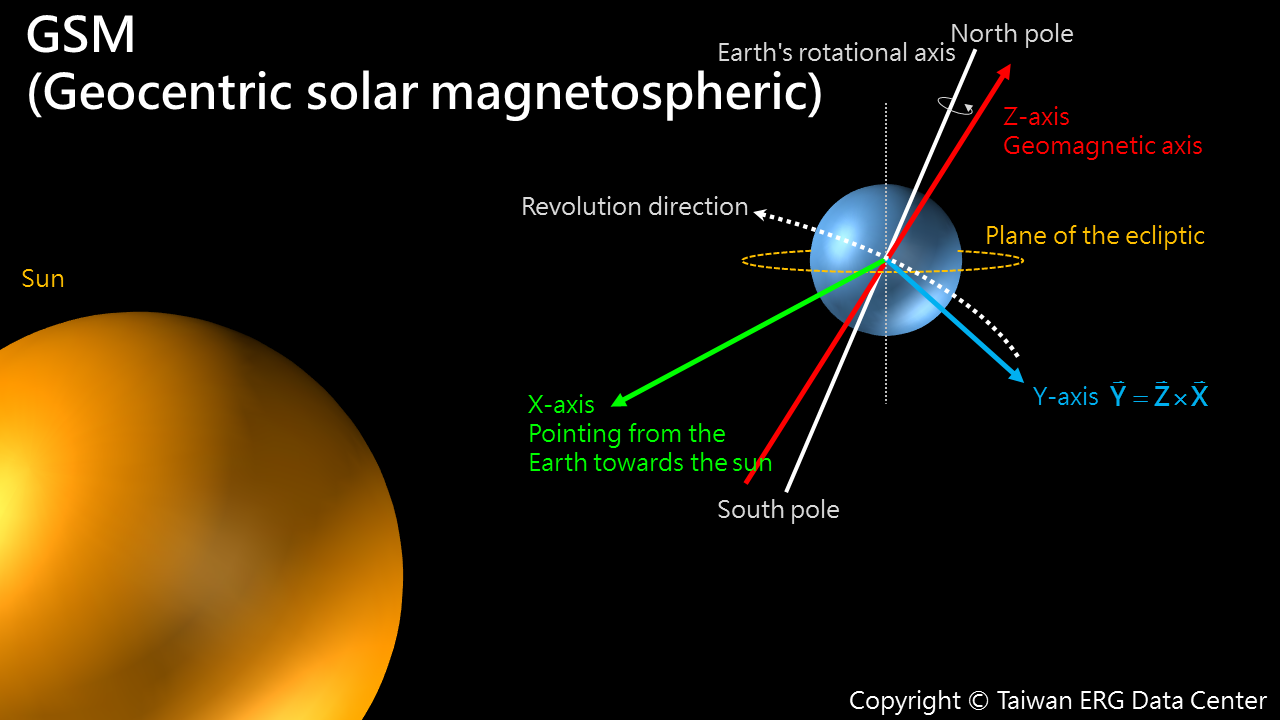
\includegraphics[width=\textwidth]{GSM.png}
    \end{minipage}
    \captionof{figure}{The GSE (left) and GSM (right) coordinate systems. Image credit: \cite{taiwanergdatacenter}.}
\end{Figure}

\subsection{The Interplanetary Magnetic Field}
Magnetic field lines are said to be ``frozen in`` to the solar wind plasma, the IMF is carried into the interplanetary region of space by solar wind from the sun. The mechanism for this is known as Alfvén's theorem, first proposed in 1942 \cite{alfven_1942}. 

DERIVE FROZEN-IN!

Because of the rotation of the sun, solar wind (along with IMF) follows a spiral pattern similar to that produced by droplets of water as a wet tennis ball is thrown into the air with rapid spin. These field lines are `open`, i.e. they have an origin, but instead of returning to a corresponding region at the opposite pole, extend indefinitely into space \cite{imfUptoLat16}. 

At the Sun's magnetic equator, field lines originating from the north and south hemispheres run parallel to each other but are oppositely directed - creating a thin current sheet known as the ``Heliospheric current sheet``. This sheet is twisted and warped due to the difference in rotational and magnetic axes and a quadrupole moment in the sun's magnetic field - it also has a spiral shape of the same form as described above \cite{alfven_1942, ParkerSpiral}.

Since the orbital plane of the Earth is located almost along the rotation axis of the sun, we experience regular shifts in the direction of flow of the IMF because the heliospheric current sheet is sometimes above and sometimes below the planet. 

When the IMF has a southward component, the northward pointing terrestrial field lines are allowed to merge in a process known as reconnection. However, when the IMF is northward, the structure of the magnetosphere is not well understood \cite{Fear1506}.

\subsection{Reconnection and Aurora}
The auroral lights, pictured in Fig.\ref{fig:auroraPic}, are a result of charged particles from the sun being accelerated towards the ionosphere - Earth's upper atmosphere - where they collide with gas molecules, each molecule causing a different colour to be emitted. 
E.g. Green (the most common colour) is caused by collisions with atomic oxygen ($557.7 nm$) \cite{hollier, BSPP}. Intense aurora will have an emission rate of several million Rayleigh ($1R=10^6 photons/cm^2s$) and most often appear as east-west aligned bands known as auroral arcs \cite{BSPP}.

\begin{Figure}
    \begin{minipage}[c]{0.67\textwidth}
        \centering
        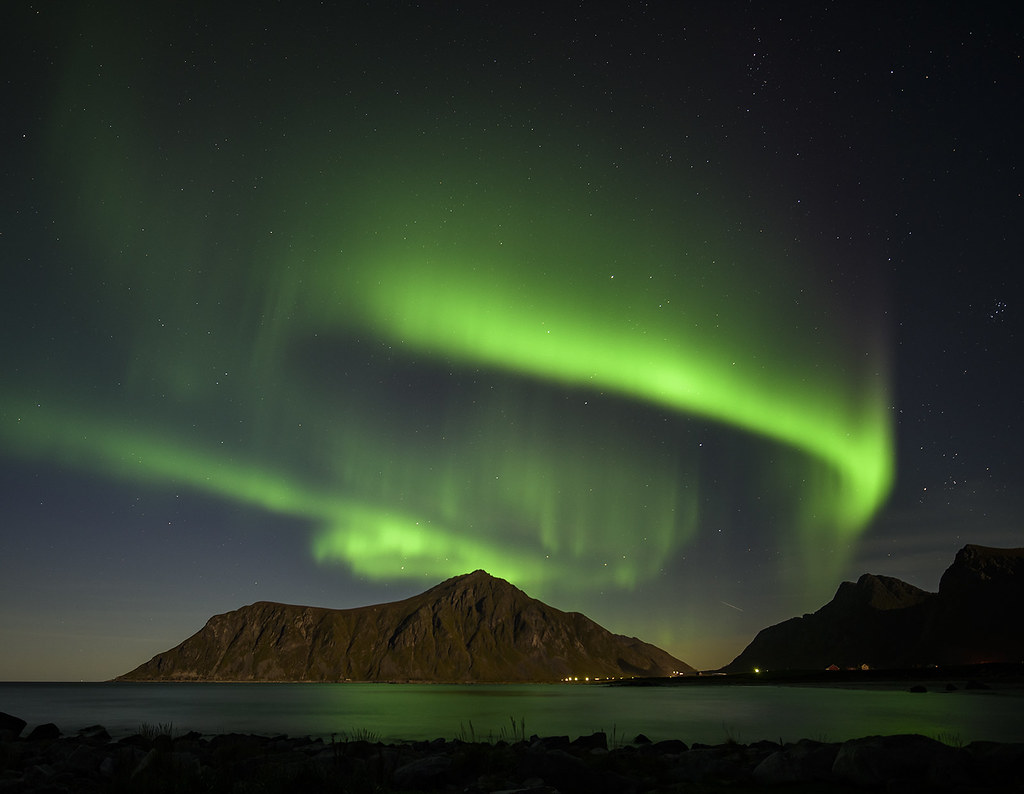
\includegraphics[width=0.8\linewidth]{nothernLights.jpg}
    \end{minipage}
    \begin{minipage}[c]{0.3\textwidth}
        \captionof{figure}{The Aurora Borealis, photographed in 2015 \cite{torino071_2015}.}
        \label{fig:auroraPic}
    \end{minipage}
\end{Figure}

Reconnection is a process that allows magnetic fields from separate domains to become joined to one another. When IMF is southward, reconnection occurs in a smooth cycle known as the Dungey cycle \cite{dungeyCycle} which is explained in Fig.\ref{fig:dungey}. Aurora is observed at latitudes of approximately $70^{\circ}$ because that is the boundary between the closed lines and the open ones at the polar cap (lobe).

\begin{Figure}
    \centering
    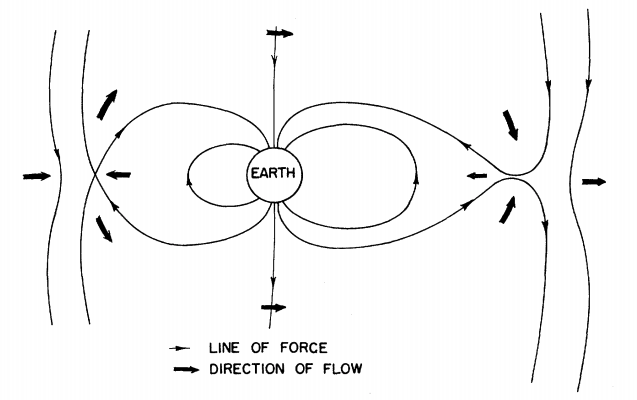
\includegraphics[width=0.6\linewidth]{dungeyCycle.png}
    \captionof{figure}{Sketch of the Dungey cycle. The IMF is assumed to be coming from the left. On the right hand side of the diagram, magnetotail reconnection is happening. Open field lines are being compressed together, eventually joining to form a closed field line that `snaps back` towards Earth, the reconnection happens typically at a radius of $\approx100R_e$. Heating and acceleration of the plasma occurs as the newly created closed field line rapidly shortens in length. The magnetic flux will then flow around to the dayside of the planet (LHS of the sketch) where it gets pushed up against the solar wind. Once again, this pressure eventually reaches a point where the field lines of the IMF and the terrestrial field merge, creating an open line with its foot on the polar cap. This line gets pushed back over to the night-side of the planet where magnetotail reconnection can happen once again (Sketch from \cite{dungeyCycle}).}
    \label{fig:dungey}
\end{Figure}

Aurora at very high latitudes are rare, but can occur in an event known as a transpolar arc \cite{polarAurora1, polarAurora2} (see figure \ref{fig:TPA}). There is much debate on their formation, one theory for their formation was proposed by Milan et al in \cite{TPAdebate}, where magnetic flux in the magnetotail lobes - the open field line region that maps down to the polar cap - reconnects but is trapped in the magnetotail. Transpolar arcs occur when the IMF is northward, which would explain why flux gets trapped in the magnetotail, there is a blockage created because dayside reconnection cannot occur.

\begin{Figure}
    \begin{minipage}[c]{0.4\textwidth}
        \centering
        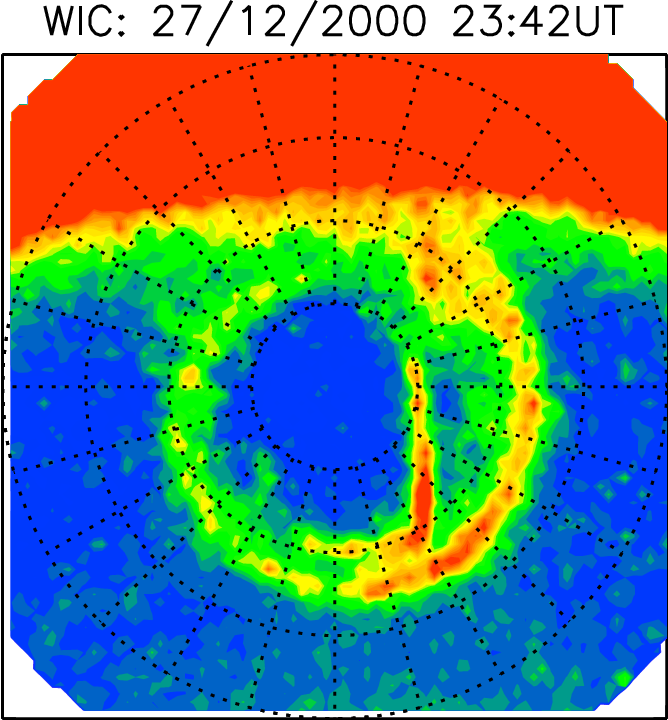
\includegraphics[width=0.9\textwidth]{transpolar_arc.png}
    \end{minipage}
    \begin{minipage}[c]{0.57\textwidth}
        \captionof{figure}{An example of a transpolar arc observed by Fear and Milan \cite{Fear2012TheID}. Dayglow is visible at the top of the image, the auroral oval is also visible as a circle in the centre of the image. The transpolar arc is the thin red band that stretches from the night side of the planet (bottom) into the polar cap region. An observer standing underneath a transpolar arc and looking up would see something that looks just like the normal aurora. The only significant difference is they are standing at a latitude that under normal circumstances would be far too high to see any aurora.}
        \label{fig:TPA}
    \end{minipage}
\end{Figure}

\section{OBSERVATIONS}
The majority of observations in this report come from Cluster, a group of four satellites built by ESA and launched in pairs on Soyuz rockets from Baikonur on the 16th July and 9th August 2000. They fly in a 57hr elliptical polar orbit and are arranged in a tetrahedron formation with a separation of between a few hundred and a few thousand km.

\subsection{Limitations of Cluster's orbit}
The orbit of cluster varies throughout the year. For significant portions of the year the satellite is well outside of the lobes, therefore the best months to extract data are July-October every year, where the spacecraft spends the majority of its time in the tail, and does not enter the magnetosheath. 

Figure \ref{fig:ClusterPos} shows Cluster's orbit through the month of September 2005 as an example, it does not cross the predicted magnetopause boundary (outer dotted parabola). Cluster will also cross through the plasmasphere in every orbit. This leaves the grey shaded region as the area of interest.

\begin{Figure}
    \begin{minipage}[c]{0.4\textwidth}
        \centering
        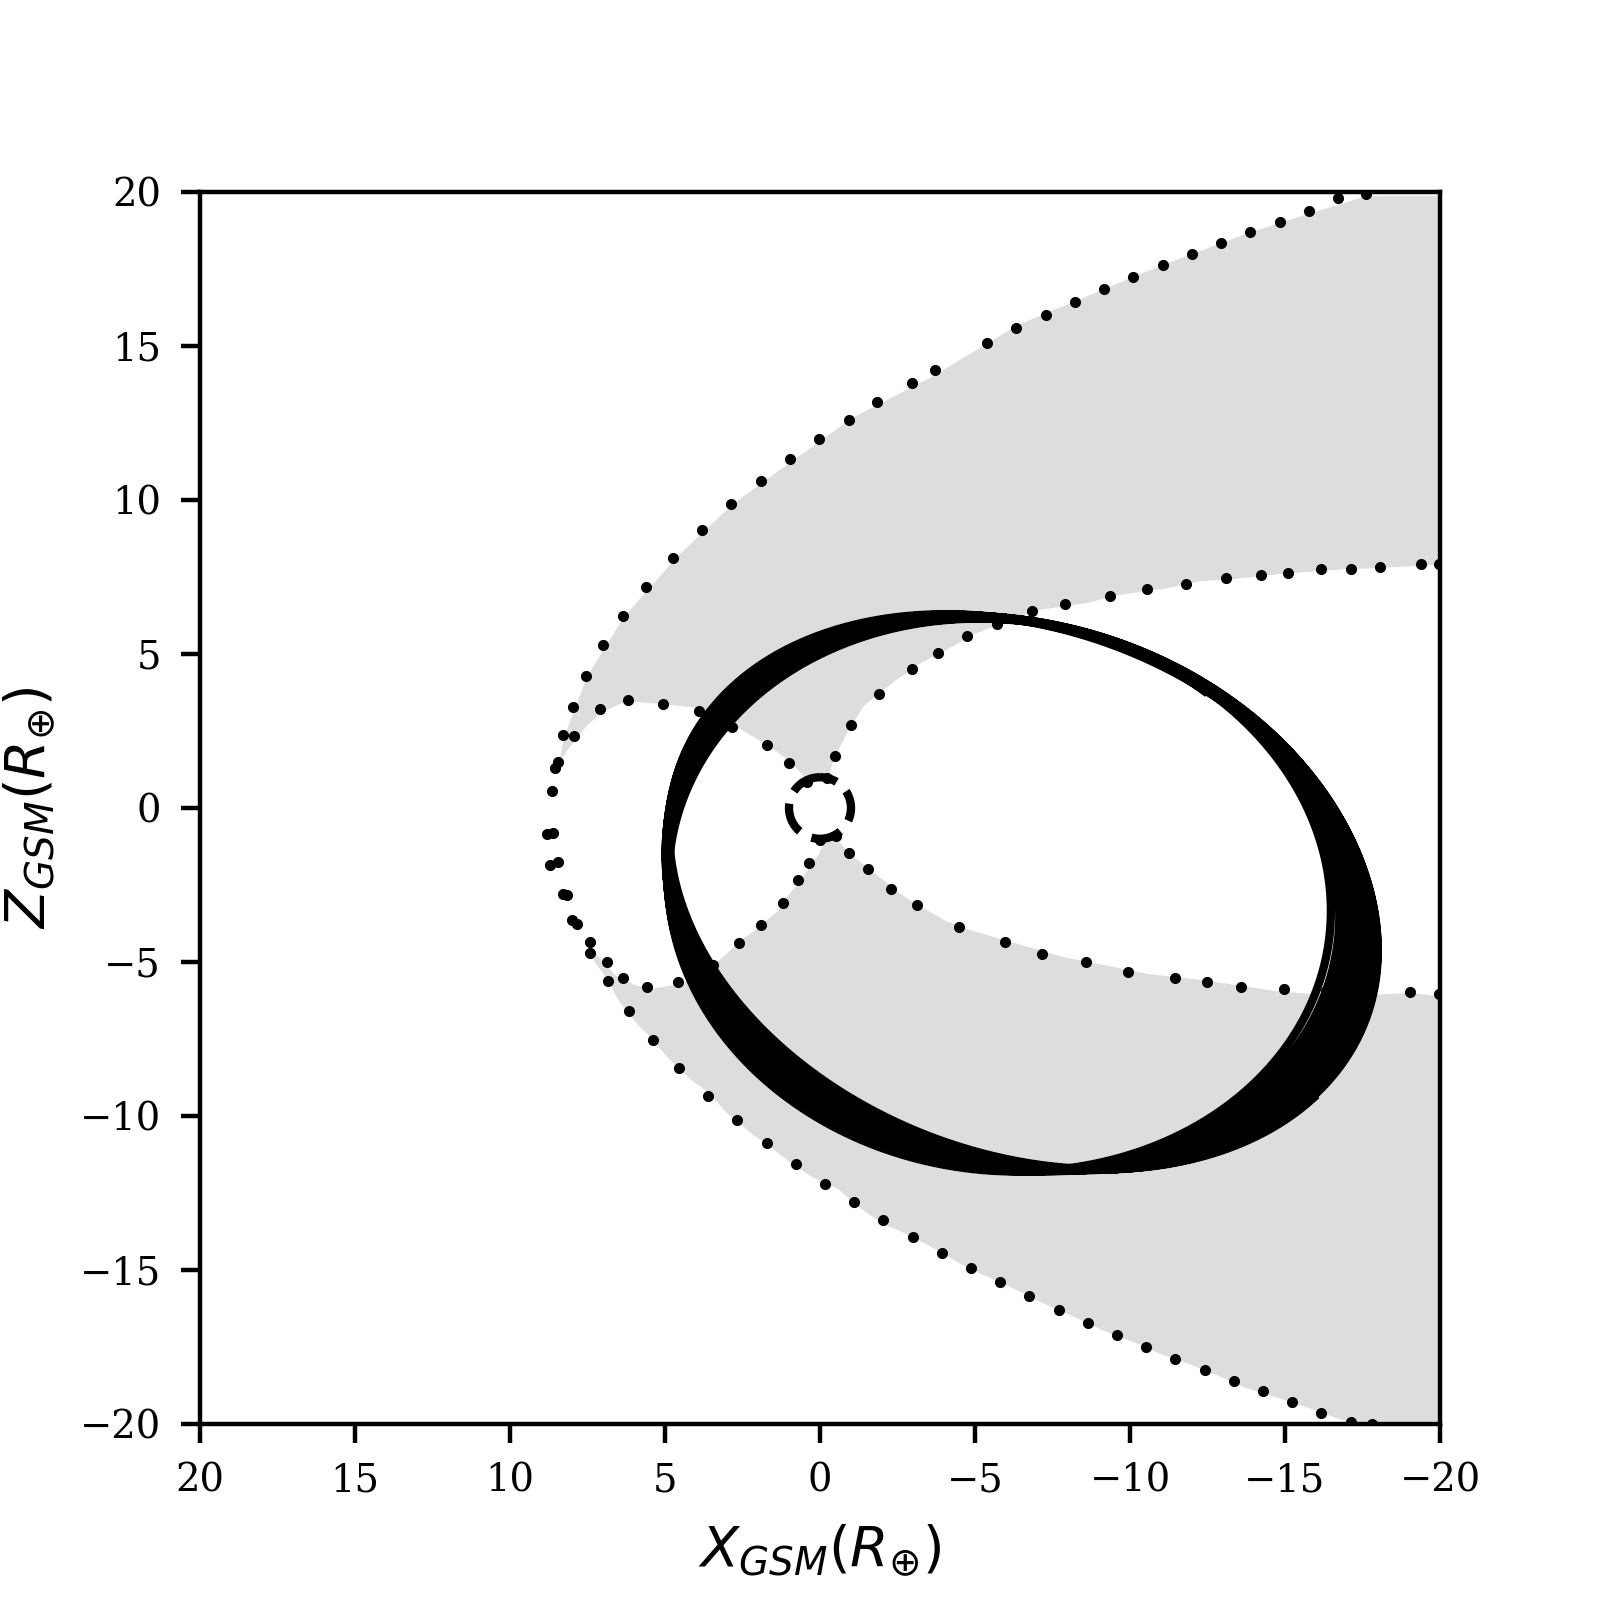
\includegraphics[width=\textwidth]{sc_pos_09_05_coloured.png}
    \end{minipage}\hfill
    \begin{minipage}[c]{0.57\textwidth}
        \captionof{figure}{Plot of Cluster's orbit throughout September 2005 (solid), along with model results for the magnetopause and open-closed boundary on 15/09/2005 (dotted) \cite{Fear1506, substormConfModel}. The grey shaded region is of interest as it contains open field lines. If a reconnection event was detected while the spacecraft was in this region then it could indicate a transpolar arc. Plotting is done in the GSM coordinate system, where +X points to the sun and +Z points along the magnetic dipole axis.}
        \label{fig:ClusterPos}
    \end{minipage}
\end{Figure}

\subsection{High temperatures in the lobe}
Occasionally when Cluster is in the lobe, it will detect periods of uncharacteristically high temperature. There is some debate on the cause of this; Shi \textit{et al} \cite{Shi2013} attribute it to solar wind penetrating into the lobe, whereas Fear \textit{et al} \cite{Fear1506} suggests that this cannot be the case due to the presence of a double loss cone. 

A double loss cone occurs when there is a magnetic mirror at both ends of the field line. This would imply that the observed field line is closed, since the Earth's dipole field has the property where magnetic field strength increases as you travel along a field line to either pole. This would cause an ion to slow down and reverse direction at the poles, i.e. it bounces back and forth from pole to pole.



\subsection{Temperature distribution in the magnetosphere}
Figure \ref{fig:tempLocations} shows the mean distribution of temperatures in the magnetosphere, during the period May to December for years 2002, 2010. We can see the general shape of the plasma sheet, a hot region to the right of the Earth where the normal aurora- generating reconnection happens.

\begin{Figure}
    \begin{minipage}[c]{0.57\textwidth}
        \centering
        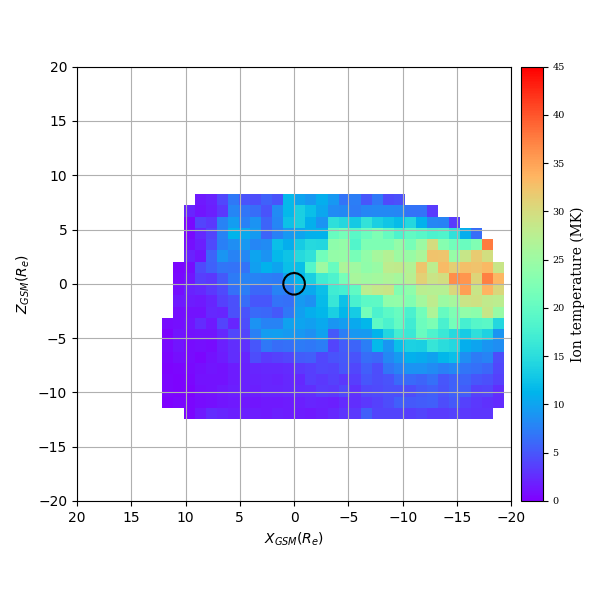
\includegraphics[width=0.9\textwidth]{tempLocations.png}
    \end{minipage}\hfill
    \begin{minipage}[c]{0.4\textwidth}
        \captionof{figure}{The temperature distribution in the magnetosphere. Measurements from Cluster orbits in the months May-December during the years 2002-2010. Each pixel is $1{R_e}^2$ in area, and represents the mean ion temperature when cluster was in that position, blue for lower temperatures and red for hotter. The plasma sheet is visible as a high temperature region to the right of Earth.}
        \label{fig:tempLocations}
    \end{minipage}
\end{Figure}

\subsection{High temperature events}
What constitutes a high temperature? That depends on where in the magnetosphere you are looking. The most easily quantifiable way to separate the plasma sheet from the lobe is to look at the Z coordinate in the Geocentric Solar Magnetospheric (GSM) coordinate system \cite{maus_2006}.

\begin{Figure}
    \begin{minipage}[c]{0.57\textwidth}
        \centering
        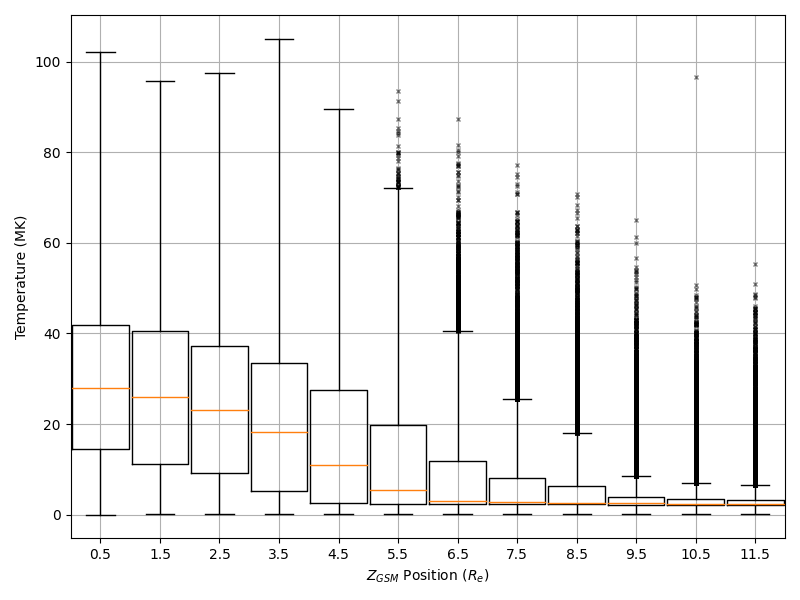
\includegraphics[width=\textwidth]{avg_temp_z.png}
    \end{minipage}\hfill
    \begin{minipage}[c]{0.4\textwidth}
        \captionof{figure}{Box plot of the temperature distribution as a function of $Z_{GSM}$. Each box covers a width of $1R_e$, starting at $[0,1)$ $R_e$ then $[1,2)$ $R_e$ etc until $[11,12]$ $R_e$. Yellow lines represent the median, each box is the interquartile range of each bin, and the ``whiskers'' are maximum and minimum values, up to $3\times IQR$. Outliers plotted as black `$\times$'. The box centred at $5.5R_e$ (for the interval $[5,6)$ $R_e$) suggests that temperatures above $\approx20MK$ are good candidates for high temperature events. Data is from Jul-Oct 2002-2010 for $X_{GSM}<0$ $R_e$.}
        \label{fig:avg_temp_z}
    \end{minipage}
\end{Figure}

We can see from Figure \ref{fig:tempLocations} that the plasma sheet ends at approximately $Z_{GSM}=\pm6R_e$. Giving an exact position for the edge of the plasma sheet is difficult as it is dynamic and in this project we were using measurements from many months and years.

In figure \ref{fig:avg_temp_z} we created a box plot of measurements from July-October 2002-2010 (for $X_{GSM} < 0$, i.e. excluding points sunwards of Earth). Taking the estimation from above that the plasma sheet ends at $\approx6R_e$, we can see from the box centred on $5.5R_e$ that temperatures exceeding $\approx 20MK$ can reasonably be considered uncharacteristically high.

\subsection{Duration of events \label{ssec:DURn}}
The event analysed by Fear \textit{et al} \cite{Fear1506} on 15-09-2005 lasted for approximately 2 hours. In figure \ref{fig:aur_comp} we analyse the length of each of our events detected in the same time period as above (Jul-Oct 2002-2010), plotting the result as a histogram. Repeating this for various cutoff points based on $|Z_{GSM}|$ gives a view of how the length of each event changes over time. 

\begin{Figure}
    \centering
    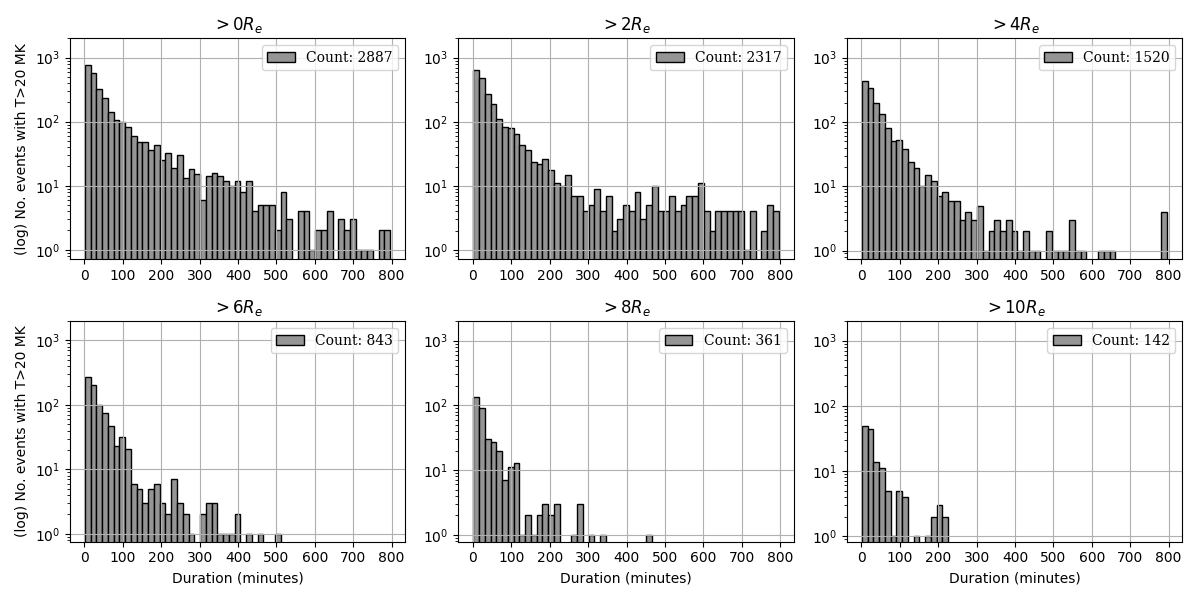
\includegraphics[width=\textwidth]{aur_comp.png}
    \captionof{figure}{Histograms showing the number of events with a certain duration (in minutes). Each panel shows a different cutoff point for $|Z_{GSM}|$. Very long duration events are consistent with passing through the plasma sheet where having a temperature above $20MK$ for over 10 hours is possible. Therefore as the $Z$ cutoff is increased we would expect those long duration events to become less common as measurements outside of the plasma sheet are excluded. What is left is $732$ (see $>6 R_e$ panel) high temperature events occurring outside the region where they are expected.}
    \label{fig:aur_comp}
\end{Figure}

We see that when the plasma sheet is excluded by excluding results where $|Z_{GSM}|<6R_e$, there are $732$ events left. This works out to be just under one per day ($732/984\approx0.75\ events/day$). The properties of this distribution are shown in table \ref{tab:event_durn}. This shows that these events are comparable in length to the 15-09-2005 event.

Many short duration events are likely to be noise. Although cluster makes a full rotation approximately every three seconds and can therefore provide measurements with similar resolution, the choice was made to average the data into five minute bins, which would match with the predicted geometric position data from \cite{cdms}, and the IMF components parameters obtained from NASA/GSFC's OMNI data set through OMNIWeb \cite{omniData}.

\begin{table}[]
    \begin{minipage}[c]{0.57\textwidth}
        \centering
        \begin{tabular}{||c|l||c|l||}
            \hline
            count & 732 & $25\%$ & 00:15:00 \\
            mean & 01:16:18 & $50\%$ & 00:25:00 \\
            std & 03:38:36 & $75\%$ & 01:00:00 \\
            min & 00:10:00 & max & 1 day 12:40:00 \\
            \hline
        \end{tabular}
    \end{minipage}\hfill
    \begin{minipage}[c]{0.4\textwidth}
        \caption{Statistical properties for the duration of events occurring at $|Z_{GSM}|>6R_e$.}
        \label{tab:event_durn}
    \end{minipage}
\end{table}

\subsection{Interplanetary Magnetic Field}
The IMF data consists of three measurements from OMNI, $B_x, B_y, B_z$, all in the GSM coordinate system.

$B_z$ represents the IMF polarity, positive northwards and negative southwards. For the time range that we have been considering, the average bz was:

\begin{equation}
    \overline{B_z} = 0.004 \pm 3.275\ nT
\end{equation}

Therefore it was effectively 50\% positive and 50\% negative. 

\section{Effect of IMF direction on temperature distribution}
Figure \ref{fig:imfDiff} shows the difference between the average temperature distribution (figure \ref{fig:tempLocations}) and an equivalent average when IMF is only northwards. Redder represents an increase in average temperature when IMF is northwards and blue is a decrease.

The interplanetary magnetic field is highly variable which has caused problems with high standard deviation throughout this project, for figure \ref{fig:imfDiff} this has resulted in a lot of noise. However, some notable features are visible. The plasma sheet is cooler during times of northward IMF, this is consistent with previous studies \cite{TAYLOR20081619} saying that the plasma sheet becomes colder and denser during extended times of northward IMF, known as the cold dense plasma sheet (CDPS).

It is also theorised that the plasma sheet expands vertically during northward IMF \cite{huang, nishida}, which could explain the increase in temperature outside of the plasma sheet.

\begin{Figure}
    \begin{minipage}[c]{0.57\textwidth}
        \centering
        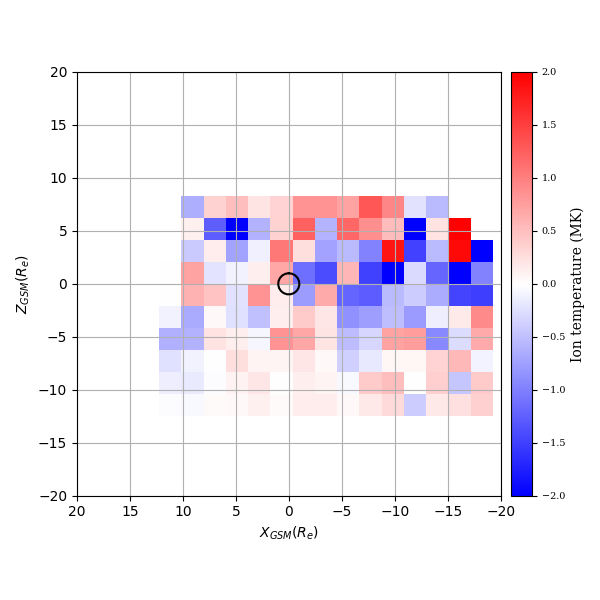
\includegraphics[width=\textwidth]{tempLocations_IMFdiff.png}
    \end{minipage}
    \begin{minipage}[c]{0.4\textwidth}
        \captionof{figure}{Difference plot of average temperature distribution (figure \ref{fig:tempLocations} compared to distribution when IMF is northward. Red indicates a higher average temperature during northward IMF and blue indicated colder. The IMF is highly variable, resulting in a lot of noise, however a decrease in temperature inside the plasma sheet and an increase above and below are still visible. This confirms other direct measurements of the plasma sheet boundary expanding vertically \cite{huang, nishida} and of the cold-dense plasma sheet formation during northward IMF. }
        \label{fig:imfDiff}
    \end{minipage}
\end{Figure}

\section{RESULTS}

\subsection{Relationship between Z and IMF direction}
If high temperatures in the lobe are caused by times of northward IMF, then we should see that the average IMF $B_Z$ increases with $Z$. 




\subsection{Connection to Transpolar Arcs}
It is possible to compare temperatures in the lobe with images of the auroral oval. As shown in section \ref{ssec:DURn}, there were 732 observed events with a temperature of over $20MK$. These can be filtered further to exclude all events with a duration less than 1.5 hours. 

This is to align with observations from SSUSI, an instrument carried on Defense Meteorological Satellite Program (DMSP) satellites that has been taking images of the auroral oval every 100 minutes since 2005. 

Computing power and internet bandwidth were limited during this project, so a full an exhaustive search of all SSUSI instrument data was not possible. Instead, we chose to limit to the F16 dataset only.

Finding a way to classify transpolar arcs automatically proved to also be beyond the scope of this project, though it would be a very interesting future extension. There is simply too much going on in the auroral oval to create an unsupervised machine learning model that distinguishes between an image of the oval that has a TPA and one that does not. A supervised model would be more useful in this instance, however a requirement for supervised learning is to have a labelled dataset to train/test on. This presents two problems:

The first is scarcity of data, there is a maximum of approximately $27,000$ images available from F16 orbits from 2005-2010 assuming F16 completes 15 orbits per day. Transpolar arcs are relatively rare, when labelling a small random sample of 100 images we found 12 that contained convincing transpolar arcs. Assuming that estimate is true for the entire sample, this leaves $3240$ images that contain a transpolar arc. Since we are trying to make a binary classification (does/doesn't have a TPA visible) and the training data needs to be balanced so that biases are not introduced, that leaves a training set of $6480$ images. The general ballpark figure for the size of supervised learning training datasets is $100,000-1,000,000$ images.

The second problem is practicality. Since this project is intended to be an analysis of data that has already been captured, it is pointless to label all historical data manually for the purposes of creating a machine learning model, as it is the labelling itself that is the goal. Though it would be useful for classifying data from future orbits.

Therefore, by filtering our high-temperature events to exclude events with a duration $< 1.5$ hours and with a height $\ge\pm7R_e$ we are left with 56 events. This is a manageable number of events to manually investigate. F16 data is organised into per-orbit files approximately 85MB in size. Downloading and analysing a file of that size with the limitations mentioned above is still to much. However, per-day quicklook plots are also available which are typically under 1MB. 

By searching for the date and time of one of the 56 high-temperature events and visually inspecting the quicklook we were able to make a judgement on whether or not there was a transpolar arc during this time.

\begin{Figure}
    \centering
    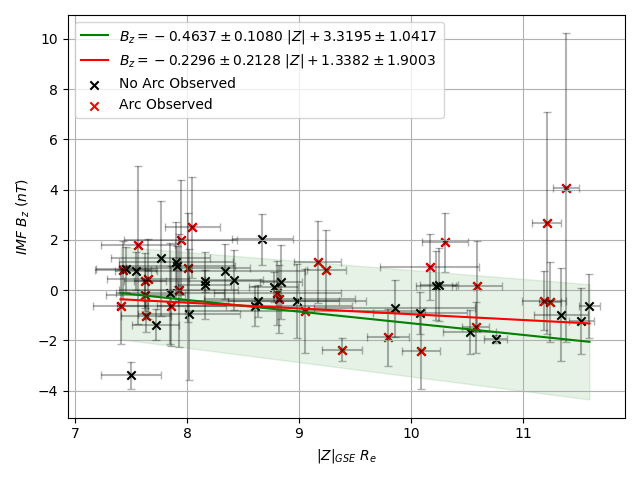
\includegraphics[width=0.7\textwidth]{tpa.png}
    \captionof{figure}{High-temperature events, a black cross shows an event where SSUSI observations did not capture a TPA, red crosses show where a TPA was observed at some point in the duration of the event. The green line is a linear fit to all the data, red line is to just events with a transpolar arc. In both cases, the best fit line is negative. This is significant because it suggests that these events are not linked to northward IMF.}
    \label{fig:tpa}
\end{Figure}

As shown in figure \ref{fig:tpa}, there was a total of 28 events that had an observed arc (exactly 50\%, 15 had IMF $> 0$). It is important to consider that SSUSI instruments do not have a wide enough field of view to capture the entire auroral oval in one pass, and that it is only over the oval for a short period of time. Also, in most cases, dayglow causes the oval at the north pole to be almost entirely obscured. This could potentially explain why there were some high-temperature events without an associated arc.

This sample size is relatively small and could be expanded upon easily by lowering the minimum acceptable length for an event. The current limit of 1.5 hours was chosen so that the F16 satellite has enough time to pass over both poles which should increase the likelihood of a TPA being observed.

However, an arc being visible in 50\% of cases does suggest a link between high-temperatures in the lobe and the formation of transpolar arcs, as it is well above the estimate quoted above of 12\%. 

There were also a large number of transpolar arcs spotted by SSUSI that were not detected by Cluster. This is easily explained by the fact that Cluster is very small and the lobe is very big, it is very likely that Cluster was just in the wrong place to be able to see it.
\section{DISCUSSION}
HI

\section{CONCLUSION: FUTURE WORK}
HI \\

\printbibliography
% \end{multicols}
\end{document}
